\chapter{Les modèles de diffusion (DDPM)}
\label{chap:ddpm}

Ce chapitre présente les \emph{Denoising Diffusion Probabilistic Models} (DDPM), introduits par
Sohl-Dickstein et al. (2015) et popularisés par Ho, Jain et Abbeel (2020) \cite{ho2020ddpm}, qui sont
à l'origine de la vague de modèles text-to-image (DALL-E~2, Imagen, Stable Diffusion).

\section{Vue d'ensemble : deux processus}

Un DDPM est défini par deux processus, tous deux des chaînes de Markov à $T$ étapes ($T \approx 1000$
en pratique) :

\begin{itemize}
    \item le \textbf{processus direct} (\emph{forward process}), noté $q$, qui bruite progressivement
    une image $x_0$ jusqu'à obtenir un bruit gaussien pur $x_T$. Ce processus est \textbf{fixé}, sans
    paramètre à apprendre ;
    \item le \textbf{processus inverse} (\emph{reverse process}), noté $p_\theta$, qui tente de défaire
    ce bruitage pas à pas. C'est ce processus, paramétré par un réseau de neurones de poids $\theta$,
    que l'on entraîne.
\end{itemize}

\begin{center}
\begin{tikzpicture}[font=\small, node distance=2.1cm]
\node (x0) {$x_0$};
\node (x1) [right=of x0] {$x_1$};
\node (dots1) [right=of x1] {$\cdots$};
\node (xt) [right=of dots1] {$x_{t-1}$};
\node (xt1) [right=of xt] {$x_t$};
\node (dots2) [right=of xt1] {$\cdots$};
\node (xT) [right=of dots2] {$x_T$};

\draw[-Stealth, bend left=25, blue!60!black] (x0) to node[above]{$q(x_1|x_0)$} (x1);
\draw[-Stealth, bend left=25, blue!60!black] (x1) to node[above]{$q$} (dots1);
\draw[-Stealth, bend left=25, blue!60!black] (dots1) to node[above]{$q$} (xt);
\draw[-Stealth, bend left=25, blue!60!black] (xt) to node[above]{$q(x_t|x_{t-1})$} (xt1);
\draw[-Stealth, bend left=25, blue!60!black] (xt1) to node[above]{$q$} (dots2);
\draw[-Stealth, bend left=25, blue!60!black] (dots2) to node[above]{$q$} (xT);

\draw[-Stealth, bend left=25, red!70!black] (x1) to node[below]{$p_\theta(x_0|x_1)$} (x0);
\draw[-Stealth, bend left=25, red!70!black] (dots1) to node[below]{$p_\theta$} (x1);
\draw[-Stealth, bend left=25, red!70!black] (xt) to node[below]{$p_\theta$} (dots1);
\draw[-Stealth, bend left=25, red!70!black] (xt1) to node[below]{$p_\theta(x_{t-1}|x_t)$} (xt);
\draw[-Stealth, bend left=25, red!70!black] (dots2) to node[below]{$p_\theta$} (xt1);
\draw[-Stealth, bend left=25, red!70!black] (xT) to node[below]{$p_\theta$} (dots2);
\end{tikzpicture}
\end{center}

\begin{center}
{\color{blue!60!black}\textbf{Forward} $q$ : bruite, fixé, va de gauche à droite} \qquad
{\color{red!70!black}\textbf{Reverse} $p_\theta$ : débruite, appris, va de droite à gauche}
\end{center}

\section{Le processus direct}

À chaque étape $t \in \{1, \dots, T\}$, on ajoute une petite quantité de bruit gaussien :
\begin{equation}
    q(x_t \mid x_{t-1}) = \mathcal{N}\!\left(x_t;\ \sqrt{1-\beta_t}\, x_{t-1},\ \beta_t I\right)
\end{equation}
où $(\beta_t)_{t=1}^T$ est un \emph{schedule de bruit} fixé à l'avance, une suite croissante de petites
valeurs (typiquement $\beta_1 = 10^{-4}$ à $\beta_T = 2 \times 10^{-2}$, croissance linéaire).

\begin{definition}[Notations usuelles]
On pose $\alpha_t = 1 - \beta_t$ et $\bar\alpha_t = \prod_{s=1}^t \alpha_s$ (produit cumulé).
\end{definition}

\subsection{Formule fermée : bruiter directement à l'étape $t$}

Le résultat clé qui rend le DDPM praticable est qu'on peut bruiter $x_0$ jusqu'à n'importe quelle étape
$t$ \textbf{sans simuler les $t-1$ étapes intermédiaires}, grâce à une propriété de composition des
lois gaussiennes :
\begin{equation}
    \boxed{q(x_t \mid x_0) = \mathcal{N}\!\left(x_t;\ \sqrt{\bar\alpha_t}\, x_0,\ (1-\bar\alpha_t) I\right)}
\end{equation}
soit, en utilisant le \emph{reparameterization trick} (écrire un tirage gaussien comme une fonction
déterministe d'un bruit standard) :
\begin{equation}
    \label{eq:qsample}
    x_t = \sqrt{\bar\alpha_t}\, x_0 + \sqrt{1-\bar\alpha_t}\, \varepsilon, \qquad \varepsilon \sim \mathcal{N}(0, I)
\end{equation}

\begin{intuition}
$\bar\alpha_t$ mesure \og combien de l'image originale reste \fg\ à l'étape $t$ : proche de $1$ pour
$t$ petit ($x_t \approx x_0$), proche de $0$ pour $t$ grand ($x_t \approx \varepsilon$, du bruit pur).
La figure~\ref{fig:noise-schedule} montre l'évolution de $\beta_t$, $\alpha_t$ et $\bar\alpha_t$ pour
le schedule utilisé dans ce projet.
\end{intuition}

\begin{figure}[h]
\centering
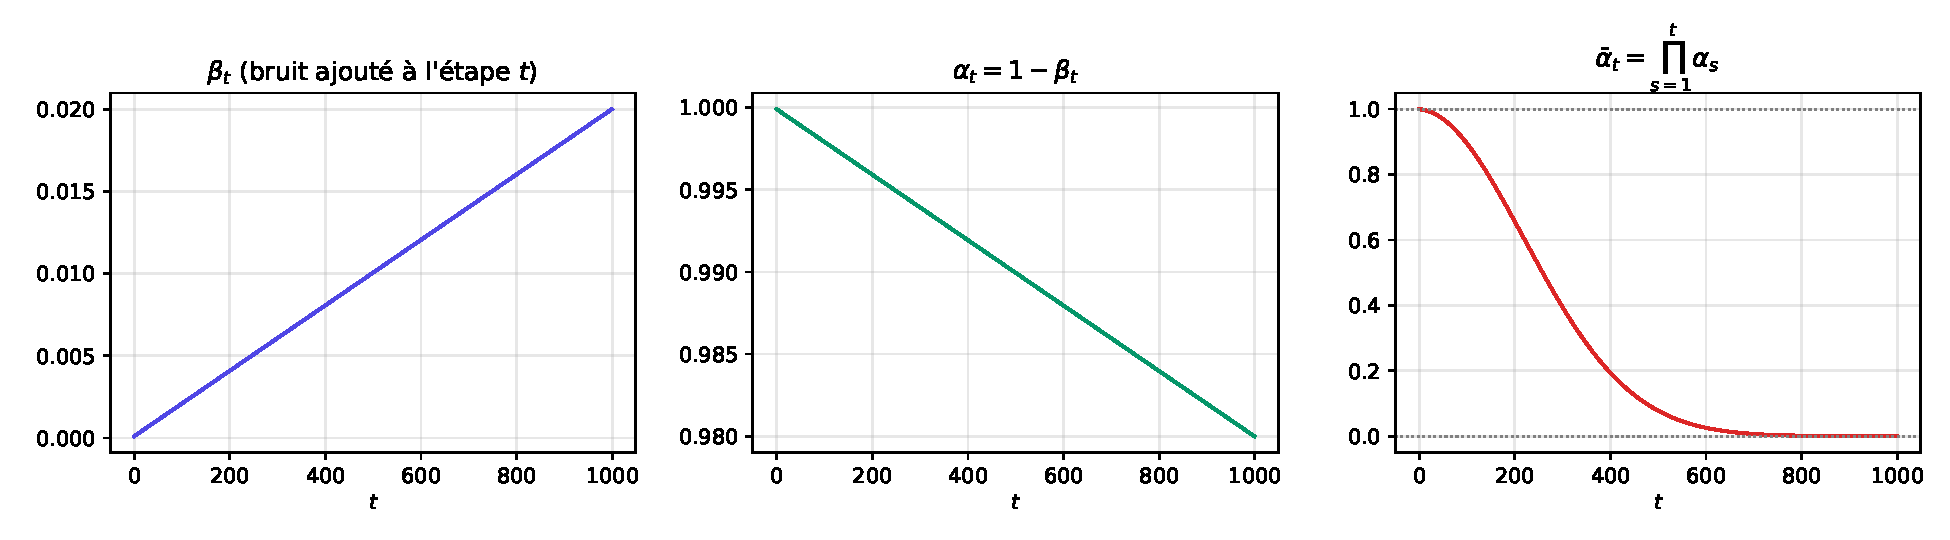
\includegraphics[width=\textwidth]{figures/noise_schedule.pdf}
\caption{Schedule de bruit linéaire ($T=1000$, $\beta_1=10^{-4}$, $\beta_T=2\times10^{-2}$). Notez
comment $\bar\alpha_t$ (produit cumulé) chute rapidement autour de $t \approx 200$–$400$ bien que
$\beta_t$ croisse linéairement : c'est un effet cumulatif, pas une propriété de $\beta_t$ lui-même.}
\label{fig:noise-schedule}
\end{figure}

\begin{figure}[h]
\centering
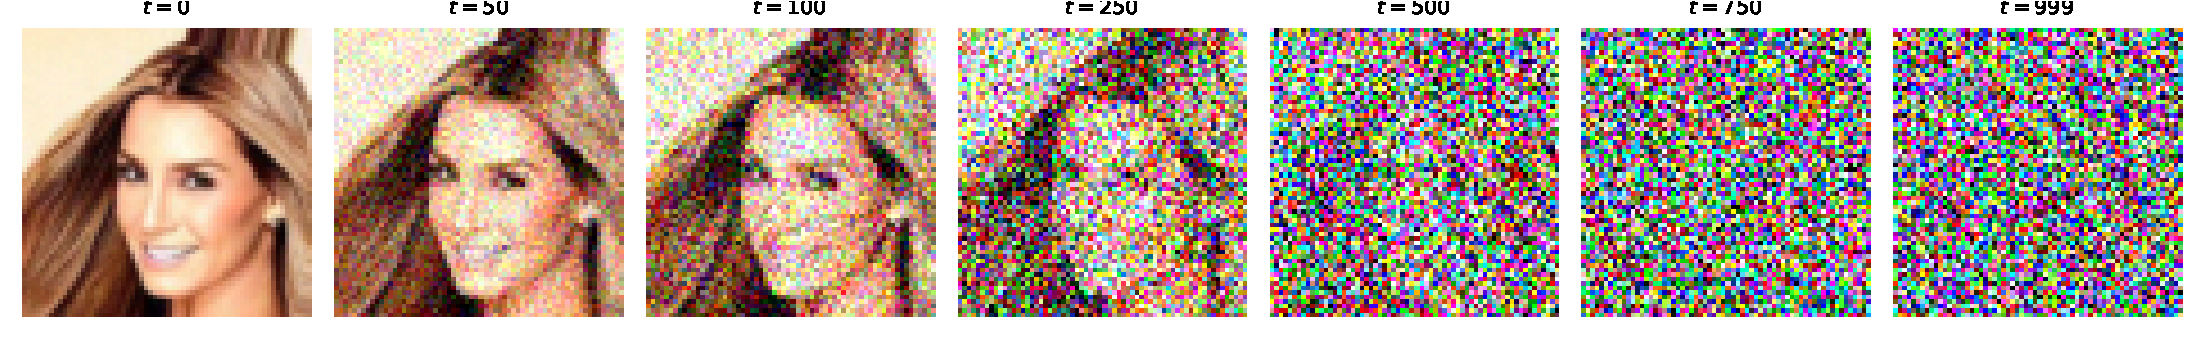
\includegraphics[width=\textwidth]{figures/forward_diffusion.pdf}
\caption{Application de la formule~\eqref{eq:qsample} à une vraie image de visage (CelebA-Dialog), pour
plusieurs valeurs de $t$. L'image reste reconnaissable jusque vers $t\approx 250$, puis se dégrade
rapidement en bruit pur — cohérent avec la chute de $\bar\alpha_t$ observée figure~\ref{fig:noise-schedule}.}
\label{fig:forward-diffusion}
\end{figure}

\section{Le processus inverse}

Défaire le bruitage revient, en théorie, à calculer $q(x_{t-1} \mid x_t)$ — mais cette distribution
dépend de $q(x_{t-1} \mid x_t, x_0)$, donc de $x_0$, que l'on ne connaît justement pas au moment de la
génération (c'est précisément ce qu'on cherche à produire). L'idée du DDPM est d'\textbf{approcher}
cette distribution inconnue par une gaussienne paramétrée :
\begin{equation}
    p_\theta(x_{t-1} \mid x_t) = \mathcal{N}\!\left(x_{t-1};\ \mu_\theta(x_t, t),\ \Sigma_\theta(x_t, t)\right)
\end{equation}
où $\mu_\theta$ est calculée par un réseau de neurones (le U-Net, chapitre~\ref{chap:architecture}), et
où $\Sigma_\theta$ est souvent fixée (non apprise) à $\sigma_t^2 I$ avec $\sigma_t^2 = \beta_t$.

\subsection{Que doit prédire le réseau ?}

Une observation cruciale simplifie tout : on peut montrer (Ho et al., 2020) que la moyenne optimale
$\mu_\theta$ s'exprime naturellement en fonction du \textbf{bruit} $\varepsilon$ qui a été ajouté à
$x_0$ pour produire $x_t$ (équation~\eqref{eq:qsample}) :
\begin{equation}
    \mu_\theta(x_t, t) = \frac{1}{\sqrt{\alpha_t}}\left(x_t - \frac{\beta_t}{\sqrt{1-\bar\alpha_t}}\,\varepsilon_\theta(x_t, t)\right)
\end{equation}
où $\varepsilon_\theta(x_t, t)$ est la sortie du réseau de neurones : \textbf{au lieu de prédire
directement $x_{t-1}$ ou $\mu_\theta$, le réseau apprend à prédire le bruit $\varepsilon$}. C'est un
choix de paramétrisation, pas une nécessité mathématique, mais Ho et al. montrent empiriquement qu'il
conduit à un entraînement bien plus stable et à de meilleurs résultats.

\begin{intuition}
Demander au réseau \og quelle image propre vois-tu dans ce bruit ? \fg\ est une question difficile et
mal posée à haut niveau de bruit (beaucoup d'images propres sont compatibles avec un $x_t$ très
bruité). Demander \og quel bruit a été ajouté ? \fg\ est une question plus simple et mieux posée :
le réseau n'a qu'à reconnaître le \emph{motif de bruit}, une tâche plus locale et plus uniforme sur
toute la plage de $t$.
\end{intuition}

Une fois qu'on a $\mu_\theta$, générer une étape du reverse process consiste à tirer :
\begin{equation}
    \label{eq:psample}
    x_{t-1} = \frac{1}{\sqrt{\alpha_t}}\left(x_t - \frac{\beta_t}{\sqrt{1-\bar\alpha_t}}\,\varepsilon_\theta(x_t, t)\right) + \sigma_t z, \qquad z \sim \mathcal{N}(0, I) \text{ si } t>0 \text{, sinon } z=0
\end{equation}

\section{La fonction de perte}

\subsection{Dérivation (aperçu)}

Comme pour un VAE, on entraîne $p_\theta$ en maximisant une borne inférieure de la log-vraisemblance
(l'ELBO), qui se décompose en une somme de termes de divergence de Kullback-Leibler entre
$q(x_{t-1}\mid x_t, x_0)$ (calculable en forme close) et $p_\theta(x_{t-1}\mid x_t)$, pour chaque $t$.
Chacun de ces termes, une fois la paramétrisation en $\varepsilon_\theta$ substituée, se réduit à une
erreur quadratique pondérée entre le bruit réel et le bruit prédit. La dérivation complète est
disponible dans \cite{ho2020ddpm} ; nous n'en retenons ici que le résultat final.

\subsection{La loss simplifiée}

Ho et al. montrent que retirer les poids issus de la dérivation théorique (c'est-à-dire utiliser une
simple MSE non pondérée) donne, en pratique, de \textbf{meilleurs} résultats visuels :
\begin{equation}
    \boxed{\mathcal{L}_{\text{simple}}(\theta) = \mathbb{E}_{t,\, x_0,\, \varepsilon}\left[\left\lVert \varepsilon - \varepsilon_\theta\!\left(\sqrt{\bar\alpha_t}\,x_0 + \sqrt{1-\bar\alpha_t}\,\varepsilon,\ t\right) \right\rVert^2\right]}
\end{equation}
avec $t \sim \mathcal{U}\{1,\dots,T\}$ et $\varepsilon \sim \mathcal{N}(0,I)$ tirés indépendamment pour
chaque exemple d'entraînement. C'est cette loss, remarquablement simple à implémenter (une MSE entre
deux tenseurs), qui est utilisée dans ce projet.

\section{Algorithmes}

\begin{codebox}[title=Algorithme 1 : Entraînement]
\textbf{répéter jusqu'à convergence :}
\begin{enumerate}[nosep]
    \item tirer $x_0 \sim p_{\text{data}}$ (un batch d'images réelles)
    \item tirer $t \sim \mathcal{U}\{1, \dots, T\}$
    \item tirer $\varepsilon \sim \mathcal{N}(0, I)$
    \item calculer $x_t = \sqrt{\bar\alpha_t}\,x_0 + \sqrt{1-\bar\alpha_t}\,\varepsilon$
    \item calculer la loss $\lVert \varepsilon - \varepsilon_\theta(x_t, t) \rVert^2$ et rétropropager
\end{enumerate}
\end{codebox}

\begin{codebox}[title=Algorithme 2 : Génération (sampling)]
\begin{enumerate}[nosep]
    \item tirer $x_T \sim \mathcal{N}(0, I)$
    \item \textbf{pour} $t = T, T-1, \dots, 1$ \textbf{faire}
    \begin{enumerate}[nosep]
        \item calculer $\varepsilon_\theta(x_t, t)$ avec le réseau entraîné
        \item calculer $x_{t-1}$ via l'équation~\eqref{eq:psample}
    \end{enumerate}
    \item retourner $x_0$
\end{enumerate}
\end{codebox}

\begin{remarque}
Contrairement à l'entraînement (un seul $t$ tiré au hasard par exemple, très rapide), la
\textbf{génération} nécessite $T$ appels séquentiels au réseau — c'est le coût principal des DDPM en
pratique, et la motivation première de méthodes comme le flow matching
(chapitre~\ref{chap:flow}) ou les schémas d'échantillonnage accélérés (DDIM, etc.), qui visent à
réduire ce nombre d'étapes.
\end{remarque}

\section{Conditionnement par texte et classifier-free guidance}
\label{sec:cfg}

Jusqu'ici, $\varepsilon_\theta(x_t, t)$ ne dépend que de l'image bruitée et du temps : le modèle est
\emph{inconditionnel}, il génère \og un visage plausible \fg\ sans contrôle sur son contenu. Pour du
text-to-image, on conditionne le réseau sur une représentation du texte $c$ (obtenue par un encodeur de
texte, voir section~\ref{sec:clip}) :
\begin{equation}
    \varepsilon_\theta(x_t, t, c)
\end{equation}
Le mécanisme précis d'injection de $c$ dans le réseau (cross-attention) est détaillé au
chapitre~\ref{chap:architecture}.

\subsection{Classifier-free guidance}

Conditionner naïvement ne garantit pas que le modèle \emph{suive fortement} le texte : rien n'empêche
le réseau d'apprendre à ignorer partiellement $c$ si les images d'entraînement sont déjà assez
prévisibles sans lui. Le \emph{classifier-free guidance} (Ho \& Salimans, 2022) \cite{ho2022cfg} est une
technique simple et efficace pour renforcer cette influence.

\textbf{À l'entraînement}, on remplace aléatoirement le conditionnement $c$ par un token vide
$\varnothing$ avec une probabilité $p_{\text{uncond}}$ (typiquement $10\,\%$), de sorte que le même
réseau apprenne \textbf{à la fois} $\varepsilon_\theta(x_t, t, c)$ (conditionnel) \textbf{et}
$\varepsilon_\theta(x_t, t, \varnothing)$ (inconditionnel).

\textbf{À la génération}, on combine les deux prédictions avec un facteur d'amplification
$w \geq 1$ (le \emph{guidance scale}) :
\begin{equation}
    \tilde\varepsilon_\theta(x_t, t, c) = \varepsilon_\theta(x_t, t, \varnothing) + w \cdot \big(\varepsilon_\theta(x_t, t, c) - \varepsilon_\theta(x_t, t, \varnothing)\big)
\end{equation}

\begin{intuition}
Le terme $\varepsilon_\theta(x_t,t,c) - \varepsilon_\theta(x_t,t,\varnothing)$ est la direction
\og apportée par le texte \fg\ : la différence entre ce que le modèle ferait avec et sans
conditionnement. L'amplifier par $w > 1$ exagère cette direction, produisant des images qui suivent le
prompt plus fidèlement — au prix, si $w$ est trop grand, d'une perte de diversité et d'artefacts
visuels (le modèle \og sur-corrige \fg).
\end{intuition}

Ce mécanisme de dropout du conditionnement à l'entraînement est implémenté dans ce projet (voir
chapitre~\ref{chap:project}) ; l'application du facteur $w$ au moment du sampling est un point
d'extension naturel du code fourni.
